\documentclass{article}
\usepackage{iclr2026_conference,times}
\usepackage{amsmath,amssymb,booktabs,graphicx,url}
\usepackage[hidelinks]{hyperref}
\iclrfinalcopy
\title{Predicting Small-Graph Random-Walk Cover Times with Four Simple Statistics}
\author{Autonomous Research Report}
\begin{document}
\maketitle
\lhead{Reproducible empirical study; not a conference submission}
\begin{abstract}
Can elementary graph statistics predict cover time more accurately than a general upper bound? We simulate 4,000 independent walks on each of 78 connected graphs with 8--28 vertices and fit a fixed log-linear ridge model using vertex count, average degree, diameter, and maximum degree. On 22 unseen graphs from familiar families, mean absolute percentage error is 15.6\%, versus 41.9\% for a fitted size-only baseline. On 12 graphs from two withheld families, error rises to 32.3\%. Monte Carlo uncertainty alone gives approximate 95\% intervals of [15.2,16.0]\% and [31.6,33.0]\%, respectively. Errors are structured: grids are overpredicted and lollipops underpredicted. The model is a useful empirical approximation on this design, not a uniform guarantee for all small graphs.
\end{abstract}

\section{Introduction}
For an undirected connected simple graph $G=(V,E)$, a simple random walk moves uniformly to a neighbor at each step. Let $T$ be the first time all vertices have been visited, counting the starting vertex at time zero. We predict
\[
 C_U(G)=\frac1n\sum_{v\in V}\mathbb E_v[T],\qquad n=|V|,
\]
so the starting vertex is uniform, rather than chosen adversarially. This distinction matters: the usual worst-start cover time $C_{\max}$ can be larger.

Classical work gives $C_U\leq C_{\max}\leq 2m(n-1)$, where $m=|E|$ \citep{aleliunas1979,lovasz1993}. Feige's asymptotically sharp worst-case bound is $(4/27+o(1))n^3$ \citep{feige1995}; its unspecified remainder does not provide a finite-$n$ numerical benchmark here. A guaranteed upper bound serves a different purpose from a fitted point estimate. We investigate the practical prediction gap, including failure cases, with a deliberately small, reproducible experiment.

\section{Method}
We compute $n$, average degree $\bar d=2m/n$, diameter $D$, and maximum degree $\Delta$. All are inexpensive for $n\leq30$; diameter uses breadth-first search from each vertex. Define $x=(\log n,\log\bar d,\log D,\log\Delta)$ and standardize each coordinate using only the training graphs. For standardized vectors $z_i$, fit
\begin{equation}
 (\hat b_0,\hat b)=\arg\min_{b_0,b}\sum_{i\in\mathcal T}
 [\log\widehat C_i-b_0-z_i^\top b]^2+\|b\|_2^2.
 \label{eq:fit}
\end{equation}
The intercept is unpenalized. The penalty is fixed at one, with no tuning, feature selection, or test-set calibration. Every training graph has equal weight. Exponentiation yields a positive point estimate; no lognormal correction is applied because graph-level residual variation is not assumed to be observation noise. The fitted equation in original units is approximately
\begin{equation}
 \widetilde C=0.8804\,n^{1.2278}\bar d^{-0.1358}D^{0.7277}\Delta^{0.3152}.
 \label{eq:model}
\end{equation}
Full-precision coefficients are saved with the results. We compare with $2m(n-1)$ and a size-only predictor $a n\log n$, whose log-scale least-squares fit on the same training set gives $a=2.8268$. These are intentionally simple benchmarks; this is not a comparison against optimized cover-time algorithms.

\section{Experiments and results}
\paragraph{Fixed graph design.}
At each $n\in\{8,12,16,20,24,28\}$ we generate one path, cycle, star, clique, and $4\times(n/4)$ rectangular grid, three independent connected Erd\H{o}s--R\'enyi graphs, and three uniform labeled trees. ER graphs use $p=3/(n-1)$ and rejection of disconnected draws. Trees use independent uniform Pr\"ufer sequences. Training uses sizes $8,12,20,24$ (44 graphs); familiar-family testing uses $16,28$ (22 graphs), combining interpolation and modest extrapolation. Entirely withheld families contribute six barbells and six lollipops, one of each per size. A barbell has two cliques of size $k=\max(3,\lfloor n/4\rfloor)$ joined through $n-2k$ internal path vertices. A lollipop has a clique of size $n/2$ joined to a path containing the other $n/2$ vertices. No test graph is isomorphic to a training graph. This is a designed collection, not a uniform sample of connected graphs.

\paragraph{Simulation and checks.}
Each graph receives 4,000 independent walks, each with a freshly sampled uniform start, without truncation. We record every walk length. For sample mean $\widehat C$ and sample standard deviation $s$, the Monte Carlo (MC) standard error is $s/\sqrt{4000}$; the approximate 95\% interval is $\widehat C\pm1.96s/\sqrt{4000}$. Across graphs its relative half-width has median 1.74\% and maximum 3.80\%. For paths, cycles and cliques, the exact uniform-start values are $(n-1)(7n-8)/6$, $n(n-1)/2$, and $(n-1)H_{n-1}$, respectively. All 18 comparisons are within 1.42 estimated standard errors. For example, the path expression follows from the expected time $i(n-1-i)$ to hit either endpoint, plus $(n-1)^2$ to cross to the other endpoint, averaged over $i$.

\begin{table}[h]
\centering\small
\begin{tabular}{lrr}\toprule
Predictor & Familiar families (22) & New families (12) \\ \midrule
Four statistics & 15.6 [10.6, 21.9] & 32.3 [19.7, 45.2] \\
Fitted $a n\log n$ & 41.9 [26.8, 59.2] & 55.5 [40.2, 69.0] \\
Upper bound $2m(n-1)$ & 1576.3 [360.4, 3555.8] & 174.1 [160.4, 188.0] \\
\bottomrule\end{tabular}

\caption{Mean absolute percentage error (MAPE), in percent. Brackets are 95\% graph-bootstrap percentile intervals conditional on the fitted model, using 4,000 resamples within each test group. They describe sensitivity to the chosen test graphs, not solely Monte Carlo error.}
\label{tab:main}
\end{table}

\paragraph{Aggregate accuracy.}
We use $100|\widetilde C_i/\widehat C_i-1|$ as each graph's absolute percentage error and average over graphs. Table~\ref{tab:main} shows that four statistics substantially improve on both baselines on this collection. The bound's very large familiar-family error is partly driven by cliques, for which it is particularly loose; the median error of the bound is still 382.1\%. The four-statistic model's median error is 12.2\% on familiar families and 30.8\% on withheld families. Its largest individual errors are 59.6\% and 68.1\%, respectively. Thus the average improvement does not mean uniformly accurate predictions.

\begin{figure}[h]
\centering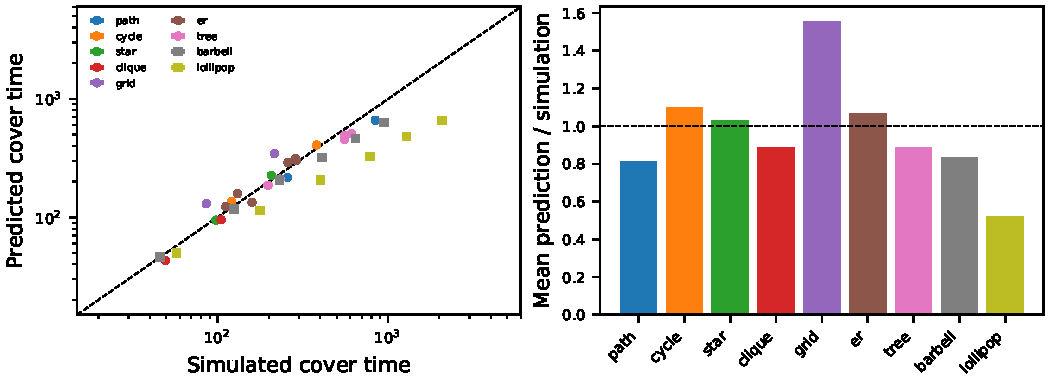
\includegraphics[width=\linewidth]{results/prediction.pdf}
\caption{Held-out graphs only. Left: predicted versus simulated cover time, with approximate 95\% MC intervals on the horizontal axis; squares mark withheld families. The dashed line is equality. Right: mean prediction-to-simulation ratio within each family.}
\label{fig:pred}
\end{figure}

\section{Discussion and limitations}
\begin{table}[h]
\centering\scriptsize\setlength{\tabcolsep}{3pt}
\begin{tabular}{lrrrrrrrrr}\toprule
Family & Path & Cycle & Star & Clique & Grid & ER & Tree & Barbell & Lollipop \\ \midrule
Count & 2 & 2 & 2 & 2 & 2 & 6 & 6 & 6 & 6 \\
Error (\%) & 18.6 & 9.8 & 6.2 & 11.2 & 55.6 & 12.1 & 11.4 & 16.8 & 47.8 \\
Bias (\%) & -18.6 & +9.8 & +2.9 & -11.2 & +55.6 & +6.7 & -11.4 & -16.6 & -47.8 \\ \bottomrule\end{tabular}

\caption{Four-statistic model by family, on held-out graphs. Error is MAPE; bias is the mean signed percentage error, $100(\widetilde C/\widehat C-1)$. Family sample sizes are very small.}
\label{tab:family}
\end{table}

\paragraph{Where prediction is reliable, and where it fails.}
On the sampled stars, cycles, cliques, ER graphs and random trees, family-average errors are between 6.2\% and 12.1\% (Table~\ref{tab:family}); paths reach 18.6\%. Grids are an important counterexample even though their family appears in training: they are overpredicted by 55.6\% on average. Lollipops, absent from training, are underpredicted by 47.8\%; barbells have 16.8\% absolute error and 16.6\% downward bias. Both the magnitude and direction of error therefore depend on family. Aggregating these families would conceal the most consequential failures.

Diameter and degree summaries omit the placement of dense regions and narrow connections. A walk can spend many steps inside a lollipop's clique before traversing its tail. This is a plausible explanation for the downward error, but the experiment does not isolate a causal mechanism: we do not hold the four features fixed while altering bottlenecks, nor test conductance or effective-resistance features. Additional structural features are a possible follow-up, not a demonstrated improvement.

\paragraph{Separating two sources of uncertainty.}
For MC-only uncertainty in the model's MAPE, we draw 2,000 independent Gaussian perturbations of every graph mean, with its estimated MC standard error, refit Equation~\ref{eq:fit} each time, and recompute errors against the perturbed test means. The resulting approximate 95\% intervals are [15.23,15.97]\% for familiar families and [31.60,33.01]\% for withheld families. This asymptotic approximation propagates fitting and evaluation noise conditional on the graph design. Its narrowness suggests that more walks alone would not resolve the main failures.

The much wider graph-resampling intervals in Table~\ref{tab:main} hold the training fit fixed and resample individual test graphs. Since families and sizes were deliberately selected, these are descriptive sensitivity intervals; they neither quantify generalization to all connected graphs nor incorporate training-graph selection uncertainty. ER and tree instances receive more aggregate weight than deterministic families. Family-specific rows should accompany any use of the aggregate score.

\paragraph{Scope.}
Only 78 graphs, nine families, and six even sizes were examined. Sizes $2$--$7$, $29$, $30$, odd sizes, other graph families, weighted or directed graphs, and worst-start cover times were not tested. For $n=1$, cover time is zero and the log model is undefined. Fixed regularization and one fixed split keep this smoke test economical but leave model-selection uncertainty unmeasured. The evidence supports a useful empirical predictor on the stated collection; it does not establish a universal error guarantee, feature sufficiency, or novelty relative to unreviewed literature.

\paragraph{Reproducibility and access restrictions.}
Code, pinned dependencies, commands, graphs, raw walks and results accompany this report (\texttt{README.md}). Master seed: 20261027. Compilation and simulation take about two CPU seconds. Only official formatting resources were consulted; no research-paper or citation-discussion pages were accessed. References were supplied in the task.

\begin{thebibliography}{3}\small
\bibitem[Aleliunas et~al.(1979)]{aleliunas1979}
R. Aleliunas, R. M. Karp, R. J. Lipton, L. Lov\'asz, and C. Rackoff.
Random walks, universal traversal sequences, and the complexity of maze problems.
In \emph{FOCS}, 1979.
\bibitem[Feige(1995)]{feige1995}
U. Feige. A tight upper bound on the cover time for random walks on graphs.
\emph{Random Structures \& Algorithms}, 1995.
\bibitem[Lov\'asz(1993)]{lovasz1993}
L. Lov\'asz. Random walks on graphs: A survey.
In \emph{Combinatorics, Paul Erd\H{o}s is Eighty}, 1993.
\end{thebibliography}
\end{document}
